
%%==================================================
%% template.tex for XMU Thesis
%% modified by miao yongchun
%% version: 1.0
%% last update: Sept. 21th, 2020
%%==================================================

% 默认单面打印 oneside 、博士论文模板 master

\documentclass[oneside, doctor]{XMU-thesis-grd}

% 模板选项: 硕士论文 master; 博士论文 doctor

\begin{document}

%%%%%%%%%%%%%%%%%%%%%%%%%%%%%%
%% 封面
%%%%%%%%%%%%%%%%%%%%%%%%%%%%%%

% 封面内容
\classification{10384}
\studentnumber{23320170155540}
\title{水下目标识别研究与应用}
\entitle{Research and Application of Underwater Target Recognition}
\author{苗永春}
\institute{\qquad}
\advisor{\qquad}
\chairman{\qquad}
\degree{工学博士}
\major{通信与信息系统}
\school{厦门大学}
\defenddate{2021 \quad 年\quad 6 月}
\submitdate{2021 \quad 年\quad 6 月}
\grantdate{2021 \quad 年\quad 9 月}
%\studentnumber{**********}

% 封面绘制
\makeInfo


% 论文原创性声明
\makeDeclareOriginal

% 论文版权声明
\makeDeclareCopyright

%%%%%%%%%%%%%%%%%%%%%%%%%%%%%%%
%%% 前置部分
%%%%%%%%%%%%%%%%%%%%%%%%%%%%%%%
\frontmatter


% 摘要
%%==================================================
%% abstract.tex for XMU Doctor Thesis
%% modified by miao yongchun
%% version: 1.0
%% last update: Sept. 21th, 2020
%%==================================================

\begin{abstract}
目前水下目标识别的应用中,主要分为两个方向,一个方向是基于被动探测,对水下声音(噪声)进行特征提取,再进行水下目标噪声的识别;另一个方向是利用成像声纳,采集到水下目标的水声图像后,对其进行图像处理以及特征提取,再使用分类器实现水下目标的识别。

\keywords{水声; 多目标识别; 应用。}
\end{abstract}

\begin{englishabstract}

   In order to exploit …….
   
\englishkeywords{Acoustic; multi-target recognition; Application}

\end{englishabstract}


%%% 符号对照表,可选,如不用可注释掉
%%%==================================================
%% denotation.tex for XMU Doctor Thesis
%% modified by miao yongchun
%% version: 1.0
%% last update: Sept. 21th, 2020
%%==================================================

\begin{denotation}
	
\item[XMU] 厦门大学的英文缩写
\item[\LaTeX] 一个很棒的排版系统
\item[\LaTeXe] 一个很棒的排版系统的最新稳定版
\item[\XeTeX] \LaTeX{}的好兄弟,事实上他有很多个兄弟,但是这个兄弟对各种语言的支持能力都很强
\item[ctex] 成套的中文\LaTeX{}解决方案,由一帮天才们开发
\item[\ce{H2SO4}] 硫酸
\item[$ e^{\pi{}i}+1=0$] 一个集自然界五大常数一体的炫酷方程
\item[\ce{2H2 + O2 -> 2H2O}] 一个昂贵的生成生命之源的方程式

\end{denotation}

% 加入中文目录
\tableofcontents

%%加入图、表索引(同时取消图表索引中章之间的垂直间隔)
%\let\origaddvspace\addvspace
%\renewcommand{\addvspace}[1]{}
%\listoffigures
%\listoftables
%\renewcommand{\addvspace}[1]{\origaddvspace{#1}}



%%%%%%%%%%%%%%%%%%%%%%%%%%%%%%
%% 正主体部分
%%%%%%%%%%%%%%%%%%%%%%%%%%%%%%
\mainmatter

%% 各章正文内容
%%==================================================
%% chapter01.tex for XMU Doctor Thesis
%% modified by miao yongchun
%% version: 1.0
%% last update: Sept. 21th, 2020
%%==================================================
\chapter{绪 论}
\echapter{Introduction}
\label{chap:intro}
\section{本论文研究的目的和意义}
\esection{The purpose of this thesis}


海洋占地球表面积的71\%,发生在海洋之中、海洋表面以及海面之上的事件在很大程度上影响着我们的生活。因此,海事遥感和监视具有重要的意义。雷达自19世纪30年代发明以来,一直在这些领域扮演着重要的角色。

……\upcite{Takahashi1996Structure,Xia2002Analysis,Jiang1989,Mao2000Motion,Feng1998}

\section{国内外研究现状及发展趋势}
\esection{development trend}

%\label{sec:***} 可标注label

\subsection{***研究现状}
\esubsection{Research status}

%\label{sec:features}
舰船和潜艇等在航行的过程中会产生较大的辐射噪声,这种噪声会以声波的形式向四周传播。由于在海水这一介质中声波有着较好的抗衰减特性,声波在水下可以较远距离地传播,这就为舰船噪声提取和目标分类识别等操作提供\cite{Jiang2005Size}。

***结果如图\ref{fig:diagram}所示

\begin{figure}
 \centering
 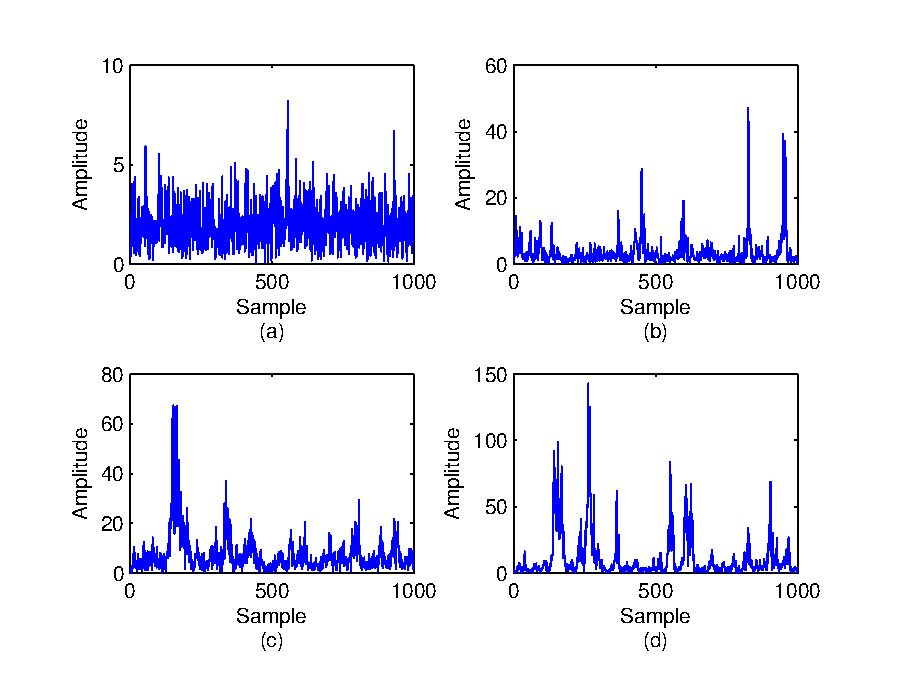
\includegraphics[width=0.75\textwidth]{figures/Fig_1_1.eps}
 \caption{**结果}\label{fig:diagram}
\end{figure}


\subsection{***研究进展}
\esubsection{Research progress}

%\label{sec:requirements}
首例***是**公司开发成功的……。

\subsection{****}
\esubsection{***}


*****************\cite{Jiang2005Size} ,如表 \ref{tab:category}所示。

\begin{table}
  \centering
  \caption{*****} \label{tab:category}
  \begin{tabular*}{0.9\textwidth}{@{\extracolsep{\fill}}cccc}
  \toprule
    1			&2		&3		&5 \\
  \midrule
    甲			&乙	    &丙		&丁 \\
    子		    &丑		&寅  	&某\\
  \bottomrule
  \end{tabular*}
\end{table}

********。
……


%%==================================================
%% chapter01.tex for XMU Doctor Thesis
%% modified by miao yongchun
%% version: 1.0
%% last update: Sept. 21th, 2020
%%==================================================
\chapter{绪 论}
\echapter{Introduction}
\label{chap:intro}
\section{本论文研究的目的和意义}
\esection{The purpose of this thesis}


海洋占地球表面积的71\%,发生在海洋之中、海洋表面以及海面之上的事件在很大程度上影响着我们的生活。因此,海事遥感和监视具有重要的意义。雷达自19世纪30年代发明以来,一直在这些领域扮演着重要的角色。

……\upcite{Takahashi1996Structure,Xia2002Analysis,Jiang1989,Mao2000Motion,Feng1998}

\section{国内外研究现状及发展趋势}
\esection{development trend}

%\label{sec:***} 可标注label

\subsection{***研究现状}
\esubsection{Research status}

%\label{sec:features}
舰船和潜艇等在航行的过程中会产生较大的辐射噪声,这种噪声会以声波的形式向四周传播。由于在海水这一介质中声波有着较好的抗衰减特性,声波在水下可以较远距离地传播,这就为舰船噪声提取和目标分类识别等操作提供\cite{Jiang2005Size}。

***结果如图\ref{fig:diagram}所示

\begin{figure}
 \centering
 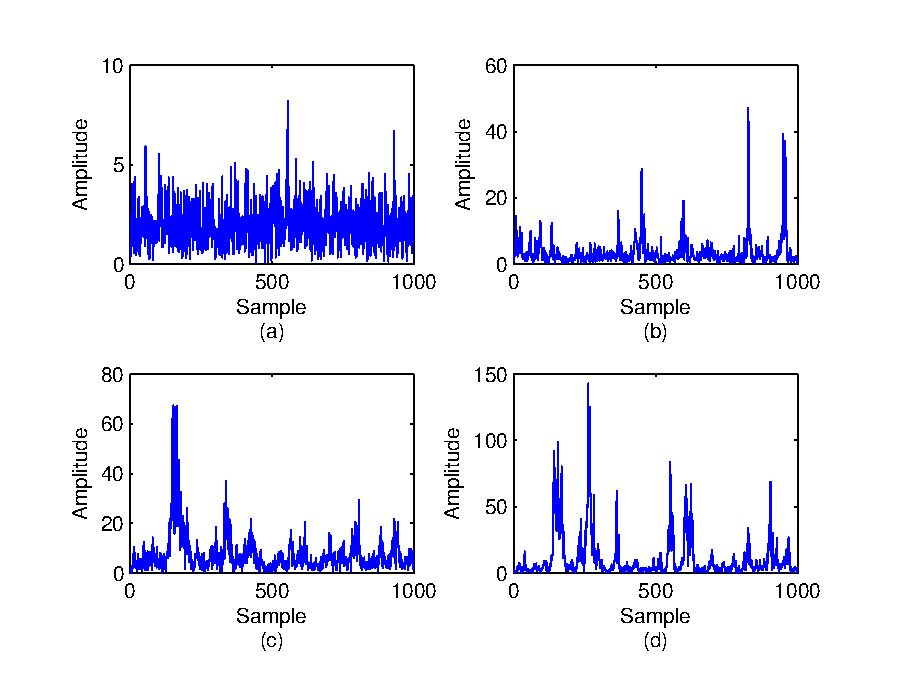
\includegraphics[width=0.75\textwidth]{figures/Fig_1_1.eps}
 \caption{**结果}\label{fig:diagram}
\end{figure}


\subsection{***研究进展}
\esubsection{Research progress}

%\label{sec:requirements}
首例***是**公司开发成功的……。

\subsection{****}
\esubsection{***}


*****************\cite{Jiang2005Size} ,如表 \ref{tab:category}所示。

\begin{table}
  \centering
  \caption{*****} \label{tab:category}
  \begin{tabular*}{0.9\textwidth}{@{\extracolsep{\fill}}cccc}
  \toprule
    1			&2		&3		&5 \\
  \midrule
    甲			&乙	    &丙		&丁 \\
    子		    &丑		&寅  	&某\\
  \bottomrule
  \end{tabular*}
\end{table}

********。
……


%\include{chapters/chapter3}

%%==================================================
%% conclusion.tex for XMU Doctor Thesis
%% modified by miao yongchun
%% version: 1.0
%% last update: Sept. 21th, 2020
%%==================================================

\chapter{结论与展望}
\echapter{Conclusions}

注释主要用于对文章篇名、作者及文内某一特定内容作必要的解释或说明。篇名、作者注置于当页地脚;对文内有关特定内容的注释可夹在文内(加圆括号),也可排在当页地脚。序号用带圆圈的阿拉伯数字表示。


%% 参考文献,五号字,使用 BibTeX,包含参考文献文件.bib

%\bibliography{reference/ref1,reference/ref2} %多个章节的参考文献
\bibliography{reference/ref1}


%%%%%%%%%%%%%%%%%%%%%%%%%%%%%%
%% 后置部分
%%%%%%%%%%%%%%%%%%%%%%%%%%%%%%

%% 附录(章节编号重新计算,使用字母进行编号)

\appendix
\renewcommand\theequation{\Alph{chapter}--\arabic{equation}}  % 附录中编号形式是"A-1"的样子
\renewcommand\thefigure{\Alph{chapter}--\arabic{figure}}
\renewcommand\thetable{\Alph{chapter}--\arabic{table}}
\renewcommand\echapter[1]{\addcontentsline{eoc}{chapter}{\protect\bf{Appendix}~\protect\numberline{\thechapter}#1}}
%%==================================================
%% app1.tex for XMU Doctor Thesis
%% modified by miao yongchun
%% version: 1.0
%% last update: Sept. 21th, 2020
%%==================================================


\chapter{***}
\echapter{***}
附录相关内容…
 
%%==================================================
%% app2.tex for XMU Doctor Thesis
%% modified by miao yongchun
%% version: 1.0
%% last update: Sept. 21th, 2020
%%==================================================

\chapter{复ARMA(2,2)-GARCH(1,1)平稳条件推导}
\echapter{**}

$\varphi (z)=0$和$\psi (z)=0$的所有根必须落在单位圆之外。将$\{ {\varphi _i}\} _{i = 1}^2$和$\{ {\psi _i}\} _{i = 1}^2$写为
\begin{align}
{\varphi _i} &= {a_i} + j{b_i} \label{eq:e1} \\
{\psi _i} &= {c_i} + j{d_i} \label{eq:e2}
\end{align}
考虑$\varphi (x)=0$,我们有
\begin{align}
{\mathop{\rm Re}\nolimits} ({x_1}) =&  - \frac{{{b_2}}}{{2(a_2^2 + b_2^2)}}\sqrt[4]{{{{\left( {a_1^2 - b_1^2 + 4{a_2}} \right)}^2} + {{\left( {2{a_1}{b_1} + 4{b_2}} \right)}^2}}} \notag \\
& \times \sin \left( {\frac{1}{2}\arg \left( {a_1^2 - b_1^2 + 4{a_2} + j(2{a_1}{b_1} + 4{b_2})} \right)} \right) \notag \\
& - \frac{{{a_2}}}{{2(a_2^2 + b_2^2)}}\sqrt[4]{{{{\left( {a_1^2 - b_1^2 + 4{a_2}} \right)}^2} + {{\left( {2{a_1}{b_1} + 4{b_2}} \right)}^2}}} \notag \\
& \times \cos \left( {\frac{1}{2}\arg \left( {a_1^2 - b_1^2 + 4{a_2} + j(2{a_1}{b_1} + 4{b_2})} \right)} \right) \notag \\
& - \frac{{{a_1}{a_2} + {b_1}{b_2}}}{{2\left( {a_2^2 + b_2^2} \right)}}  \label{eq:e3}
\end{align}
\begin{align}
{\mathop{\rm Im}\nolimits} ({x_1}) =&  - \frac{{{a_2}}}{{2(a_2^2 + b_2^2)}}\sqrt[4]{{{{\left( {a_1^2 - b_1^2 + 4{a_2}} \right)}^2} + {{\left( {2{a_1}{b_1} + 4{b_2}} \right)}^2}}} \notag \\
& \times \sin \left( {\frac{1}{2}\arg \left( {a_1^2 - b_1^2 + 4{a_2} + j(2{a_1}{b_1} + 4{b_2})} \right)} \right) \notag \\
& + \frac{{{b_2}}}{{2(a_2^2 + b_2^2)}}\sqrt[4]{{{{\left( {a_1^2 - b_1^2 + 4{a_2}} \right)}^2} + {{\left( {2{a_1}{b_1} + 4{b_2}} \right)}^2}}} \notag \\
& \times \cos \left( {\frac{1}{2}\arg \left( {a_1^2 - b_1^2 + 4{a_2} + j(2{a_1}{b_1} + 4{b_2})} \right)} \right) \notag \\
& + \frac{{{a_1}{b_2} - {a_2}{b_1}}}{{2\left( {a_2^2 + b_2^2} \right)}}  \label{eq:e4}
\end{align}
\begin{align}
{\mathop{\rm Re}\nolimits} ({x_2}) =&   \frac{{{b_2}}}{{2(a_2^2 + b_2^2)}}\sqrt[4]{{{{\left( {a_1^2 - b_1^2 + 4{a_2}} \right)}^2} + {{\left( {2{a_1}{b_1} + 4{b_2}} \right)}^2}}} \notag \\
& \times \sin \left( {\frac{1}{2}\arg \left( {a_1^2 - b_1^2 + 4{a_2} + j(2{a_1}{b_1} + 4{b_2})} \right)} \right) \notag \\
& + \frac{{{a_2}}}{{2(a_2^2 + b_2^2)}}\sqrt[4]{{{{\left( {a_1^2 - b_1^2 + 4{a_2}} \right)}^2} + {{\left( {2{a_1}{b_1} + 4{b_2}} \right)}^2}}} \notag \\
& \times \cos \left( {\frac{1}{2}\arg \left( {a_1^2 - b_1^2 + 4{a_2} + j(2{a_1}{b_1} + 4{b_2})} \right)} \right) \notag \\
& - \frac{{{a_1}{a_2} + {b_1}{b_2}}}{{2\left( {a_2^2 + b_2^2} \right)}}\label{eq:e5}
\end{align}
\begin{align}
{\mathop{\rm Im}\nolimits} ({x_2}) =&   \frac{{{a_2}}}{{2(a_2^2 + b_2^2)}}\sqrt[4]{{{{\left( {a_1^2 - b_1^2 + 4{a_2}} \right)}^2} + {{\left( {2{a_1}{b_1} + 4{b_2}} \right)}^2}}} \notag \\
& \times \sin \left( {\frac{1}{2}\arg \left( {a_1^2 - b_1^2 + 4{a_2} + j(2{a_1}{b_1} + 4{b_2})} \right)} \right) \notag \\
& - \frac{{{b_2}}}{{2(a_2^2 + b_2^2)}}\sqrt[4]{{{{\left( {a_1^2 - b_1^2 + 4{a_2}} \right)}^2} + {{\left( {2{a_1}{b_1} + 4{b_2}} \right)}^2}}} \notag \\
& \times \cos \left( {\frac{1}{2}\arg \left( {a_1^2 - b_1^2 + 4{a_2} + j(2{a_1}{b_1} + 4{b_2})} \right)} \right) \notag \\
& + \frac{{{a_1}{b_2} - {a_2}{b_1}}}{{2\left( {a_2^2 + b_2^2} \right)}}\label{eq:e6}
\end{align}
类似地,考虑$\psi (z)=0$,我们有
\begin{align}
{\mathop{\rm Re}\nolimits} ({z_1}) =&  - \frac{{{d_2}}}{{2(c_2^2 + d_2^2)}}\sqrt[4]{{{{\left( {c_1^2 - d_1^2 - 4{c_2}} \right)}^2} + {{\left( {2{c_1}{d_1} - 4{d_2}} \right)}^2}}} \notag \\
& \times \sin \left( {\frac{1}{2}\arg \left( {c_1^2 - d_1^2 - 4{c_2} + j(2{c_1}{d_1} - 4{d_2})} \right)} \right) \notag \\
& - \frac{{{c_2}}}{{2(c_2^2 + d_2^2)}}\sqrt[4]{{{{\left( {c_1^2 - d_1^2 - 4{c_2}} \right)}^2} + {{\left( {2{c_1}{d_1} - 4{d_2}} \right)}^2}}} \notag \\
& \times \cos \left( {\frac{1}{2}\arg \left( {c_1^2 - d_1^2 - 4{c_2} + j(2{c_1}{d_1} - 4{d_2})} \right)} \right) \notag \\
& - \frac{{{c_1}{c_2} + {d_1}{d_2}}}{{2\left( {c_2^2 + d_2^2} \right)}}  \label{eq:e7}
\end{align}
\begin{align}
{\mathop{\rm Im}\nolimits} ({z_1}) =&  - \frac{{{c_2}}}{{2(c_2^2 + d_2^2)}}\sqrt[4]{{{{\left( {c_1^2 - d_1^2 - 4{c_2}} \right)}^2} + {{\left( {2{c_1}{d_1} - 4{d_2}} \right)}^2}}} \notag \\
& \times \sin \left( {\frac{1}{2}\arg \left( {c_1^2 - d_1^2 - 4{c_2} + j(2{c_1}{d_1} - 4{d_2})} \right)} \right) \notag \\
& + \frac{{{d_2}}}{{2(c_2^2 + d_2^2)}}\sqrt[4]{{{{\left( {c_1^2 - d_1^2 - 4{c_2}} \right)}^2} + {{\left( {2{c_1}{d_1} - 4{d_2}} \right)}^2}}} \notag \\
& \times \cos \left( {\frac{1}{2}\arg \left( {c_1^2 - d_1^2 - 4{c_2} + j(2{c_1}{d_1} - 4{d_2})} \right)} \right) \notag \\
& + \frac{{{c_1}{d_2} - {c_2}{d_1}}}{{2\left( {c_2^2 + d_2^2} \right)}}  \label{eq:e8}
\end{align}
\begin{align}
{\mathop{\rm Re}\nolimits} ({z_2}) =&   \frac{{{d_2}}}{{2(c_2^2 + d_2^2)}}\sqrt[4]{{{{\left( {c_1^2 - d_1^2 - 4{c_2}} \right)}^2} + {{\left( {2{c_1}{d_1} - 4{d_2}} \right)}^2}}} \notag \\
& \times \sin \left( {\frac{1}{2}\arg \left( {c_1^2 - d_1^2 - 4{c_2} + j(2{c_1}{d_1} - 4{d_2})} \right)} \right) \notag \\
& + \frac{{{c_2}}}{{2(c_2^2 + d_2^2)}}\sqrt[4]{{{{\left( {c_1^2 - d_1^2 - 4{c_2}} \right)}^2} + {{\left( {2{c_1}{d_1} - 4{d_2}} \right)}^2}}} \notag \\
& \times \cos \left( {\frac{1}{2}\arg \left( {c_1^2 - d_1^2 - 4{c_2} + j(2{c_1}{d_1} - 4{d_2})} \right)} \right) \notag \\
& - \frac{{{c_1}{c_2} + {d_1}{d_2}}}{{2\left( {c_2^2 + d_2^2} \right)}}  \label{eq:e9}
\end{align}
\begin{align}
{\mathop{\rm Im}\nolimits} ({z_2}) =&   \frac{{{c_2}}}{{2(c_2^2 + d_2^2)}}\sqrt[4]{{{{\left( {c_1^2 - d_1^2 - 4{c_2}} \right)}^2} + {{\left( {2{c_1}{d_1} - 4{d_2}} \right)}^2}}} \notag \\
& \times \sin \left( {\frac{1}{2}\arg \left( {c_1^2 - d_1^2 - 4{c_2} + j(2{c_1}{d_1} - 4{d_2})} \right)} \right) \notag \\
& - \frac{{{d_2}}}{{2(c_2^2 + d_2^2)}}\sqrt[4]{{{{\left( {c_1^2 - d_1^2 - 4{c_2}} \right)}^2} + {{\left( {2{c_1}{d_1} - 4{d_2}} \right)}^2}}} \notag \\
& \times \cos \left( {\frac{1}{2}\arg \left( {c_1^2 - d_1^2 - 4{c_2} + j(2{c_1}{d_1} - 4{d_2})} \right)} \right) \notag \\
& + \frac{{{c_1}{d_2} - {c_2}{d_1}}}{{2\left( {c_2^2 + d_2^2} \right)}}  \label{eq:e10}
\end{align}
其中,${\mathop{\rm Re}\nolimits} ( \cdot )$和${\mathop{\rm Im}\nolimits} ( \cdot )$分别表示对复数取实部和虚部,$\arg ( \cdot )$表示角度。因此,复ARMA(2,2)-GARCH(1,1)的平稳条件可以写为
\begin{align}
&{\mathop{\rm Re}\nolimits} {({x_1})^2} + {\mathop{\rm Im}\nolimits} {({x_1})^2} > 1 \label{eq:e11} \\
&{\mathop{\rm Re}\nolimits} {({x_2})^2} + {\mathop{\rm Im}\nolimits} {({x_2})^2} > 1 \label{eq:e12}\\
&{\mathop{\rm Re}\nolimits} {({z_1})^2} + {\mathop{\rm Im}\nolimits} {({z_1})^2} > 1 \label{eq:e13}\\
&{\mathop{\rm Re}\nolimits} {({z_2})^2} + {\mathop{\rm Im}\nolimits} {({z_2})^2} > 1 \label{eq:e14}
\end{align}
 

%(其后部分无编号)
\backmatter

% 发表文章目录
%%==================================================
%% pub.tex for XMU Doctor Thesis
%% modified by miao yongchun
%% version: 1.0
%% last update: Sept. 21th, 2020
%%==================================================

\begin{publications}{99}

    \item{Yongchun Miao, Haixin Sun and Jie Qi}. {Synchro-Compensating Chirplet Transform}[J]. IEEE Signal Processing Letters 25(9), 2018, 1413-1417.(SCI)

\end{publications}

% 致谢
%%==================================================
%% thanks.tex for XMU Doctor Thesis
%% modified by miao yongchun
%% version: 1.0
%% last update: Sept. 21th, 2020
%%==================================================

\begin{thanks}

本论文的工作是在导师……。

\end{thanks}



\end{document}
